\chapter{Uranium Enrichment Regression Results and Discussion}

% https://www.ncbi.nlm.nih.gov/pmc/articles/PMC5554294/

% great examples of various enriched U with a large range of detector resolutions https://www.lanl.gov/orgs/n/n1/docs/la_14206.pdf

% u232 origin, enrichment as function of u235 fraction https://www.pnnl.gov/main/publications/external/technical_reports/PNNL-12075.pdf

% Although mass spectrometry leads to very accurate analytical results, it has the drawbacks of high costs of the device and its operation involving a long process and destructive sample analysis [1], [2]. https://www.sciencedirect.com/science/article/pii/S1738573317308057#bib1

Verifying the enrichment of HEU through passive nondestructive analysis is important for safeguards applications and homeland security tasks. Nondestructive analysis is preferred to preserve forensics evidence and to allow for remote measurements. Measurements of materials with unknown enrichment, shielding, and geometry are typically performed with high resolution HPGe detectors using the Multi-Group Analysis for Uranium (MGAU) software \cite{MGAU1994}. The traditional method for using NaI detectors to measure uranium enrichment is the enrichment meter method \cite{Reilly1970}. This method exploits the proportionality between the activity of the 186 keV photon and the enrichment of $^{235}$U. The enrichment meter method works by finding calibration constants that relate counts in two ROI's (one around the 186 keV peak and one in the background region to the right of the peak) to the enrichment,
%
\begin{equation} \label{eq:enrichment_meter_principle}
E = A * ROI1 + B * ROI2.
\end{equation}
%
The ROI's. Finding these constants requires measuring two known uranium enrichment standards in the same configuration. It is possible to extend this method to other shielding configurations, but this introduces a risk of adding systematic errors. An automated version of this method called NaIGEM (NaI Gamma Enrichment Measurements) is included in the HM-5 instrument used by the IAEA \cite{MORTREAU2004}.


% Measuring the enrichment of uranium is made difficult by the fact that it's characteristic gamma-rays are easily shielded. This task is made more difficult for treaty verification by the restriction placed on inspectors. IAEA inspectors face two major restrictions: a limited amount of time to measure data from declared items and the requirement for an information barrier. This means that direct viewing and analysis of the gamma-ray spectrum - necessary for the enrichment meter method - is impossible. 


% "Generally, low resolution measurements of 'clean' uranium can be made to 1\% precision over nearly the entire range of uranium enrichment. Measurements in both Europe and the Former Soviet Union have observed bias effects of 5-10\% in low-resolution measurements caused by minor isotopes of uranium. This level of bias has been deemed unacceptable, causing some inspectors to resort to more expensive, time-consuming alternatives like mass spectrometry or liquid-nitrogen-cooler high-resolution detectors. As the international safeguards community attempts to inspect more facilities with less resources, these alternatives become highly undesirable. The minor isotopes come from the use of uranium recycled from reactors being used as feed in the enrichment plants. Daughters of $^{232}$U or $^{236}$U include the thorium decay chain which emits a 238.6-keV gamma ray from $^{212}$Pb. This gamma ray falls in the ROI used to estimate the Compton continuum under the 186-keV gamma ray. In addition, the multitude of high-energy gamma rays from the daughters of $^{232}$U change the shape of the Compton continuum that lies under the desired 186-keV peak. Just to make the entire issue more challenging, the level of this interference varies widely among the samples generally offered to the inspector, causing unpredictable, wide variations in the bias effects" \cite{SPRINKLE1997}

% Accuracies of +/- 10\% are expected for quick checks of high enriched material while accuracies of +/- 1\% are expected to verify mass spectroscopy measurments \cite{Kull1974}.

% Need to address sample wall effect

% Changes in background in the facility may affect performance. Studies done measuring uranium enrichment in marine environments have shown that background radiation is important and that existing methods  \cite{Hofstetter2008}.


% \begin{figure}[H]
% 	\centering
% 	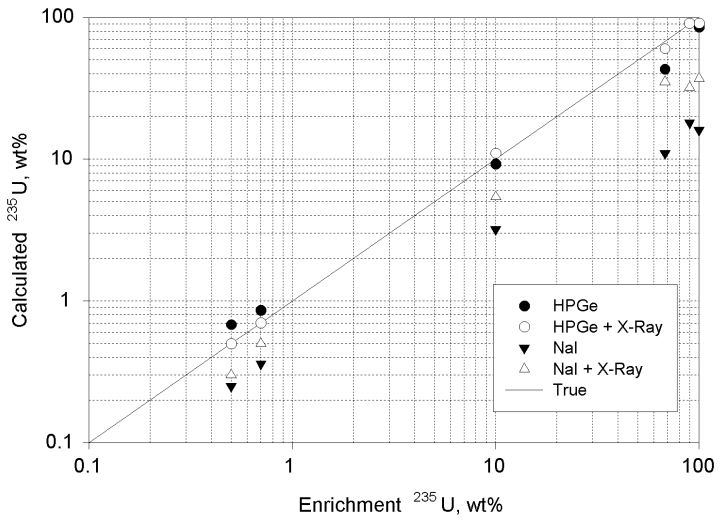
\includegraphics[width=0.99\linewidth]{images/GADRAS_enrichment_hofstetter}
% 	\caption{Uranium isotopic enrichments calculated from GADRASw analysis of HPGe and NaI spectra with and without additional uranium X-ray component. Reproduced from \cite{Hofstetter2008}}.
% 	\label{fig:GADRAS_enrichment_hofstetter}
% \end{figure}


\section{Problem Description and Training Dataset Overview}

The gamma-ray signatures from HEU come from the decay of $^{238}$U, $^{235}$U, $^{232}$U, and the daughters of these isotopes. In low-resolution detectors, The primary photopeaks of $^{235}$U signature are at 144 keV, 163 keV, and 186 keV. The $^{238}$U daughter $^{234m}$Pa produces two main photopeaks at 766 keV and 1001 keV. $^{232}$U, only present in significant quantities in recycled uranium, produces a photopeak at 2614 keV from its $^{208}$Tl daughter. 

% u232 production reactions from uranium species https://www.pnnl.gov/main/publications/external/technical_reports/PNNL-12075.pdf

% FRAM application to U and Pu isotopics https://www.lanl.gov/orgs/n/n1/appnotes/LA-14018-M.pdf

\subsection{Training Datasets}

The software package RadSrc was used to generate the specific gamma-ray intensities for $^{235}$U, $^{238}$U, and $^{232}$U templates \cite{Hiller2007}. RadSrc, developed at Lawrence Livermore National Laboratory, uses Bateman equations to calculate in-growth of daughters and their respective specific gamma-ray intensities. Isotopes in enriched uranium reach secular equilibrium in about six months. To account for this, RadSrc was used to find specific gamma-ray intensities for 50 year old uranium species. The specific activities for each species are found in Table \ref{table:specific_activities_radsrc}.

A coupled MCNP (Monte Carlo N-Particle Transport Code) and GADRAS-DRF code was used to simulate the spectrum from each uranium isotope uniformly distributed in a solid 13 kg uranium sphere. The MCNP code was used to calculate the physics due to self attenuation and distance and GADRAS-DRF was used to model the response in a 2'' x 2'' NaI detector. Simulation parameters are shown in Table \ref{table:hyperparameter_dataset_full_parameters_enrichment}.

The amount of each component's spectral template was combined based on a given enrichment. One study estimated that impurities of $^{232}$U with a mass fraction of 6.0E-9 existed in one sample of HEU created with recycled material \cite{RawoolSullivan2012}. Based on this, to account for various burn-up conditions in the recycled material \cite{Peurrung2019}, each sample that included $^{232}$U used a mass fraction uniformly chosen between 4e-9 and 2e-8. The probability that a spectrum was simulated with $^{232}$U was one half. 

\begin{table}[H]
\centering
\caption{Specific activities for 50 year old uranium species.}
\label{table:specific_activities_radsrc}
\begin{tabular}{cc}
% \cline{2-3}
% Isotope & photos/second/gram \\ \hline
% Isotope & $\frac{photos}{s g}$ \\ \hline
Isotope & {\begin{tabular}[c]{@{}c@{}}Specific Gamma-ray\\ Intensities [$\gamma$/gram/second]\end{tabular}} \\ \hline
% Isotope & Specific Gamma-ray Intensities [$\gamma$/gram/second] \\ \hline
\multicolumn{1}{c}{$^{232}$U} & 1.20e12 \\ 
\multicolumn{1}{c}{$^{235}$U} & 2.07e5 \\
\multicolumn{1}{c}{$^{238}$U} & 3.80e3 \\ 
\end{tabular}
\end{table}


\begin{table}[H]
\centering
\caption{Range of parameters used for the uranium enrichment dataset.}
\label{table:hyperparameter_dataset_full_parameters_enrichment}
\begin{tabular}{ccc}
% \cline{2-3}
 & Parameter Range & Sampling \\ \hline
\multicolumn{1}{c}{Source-Detector Distance {[}cm{]}} & 25, 50, 100 & Uniform \\ % \hline
\multicolumn{1}{c}{FWHM 662 keV [s]} & 6.0, 6.5, 7.0, 7.5 & N/A \\ % \hline
\multicolumn{1}{c}{\begin{tabular}[c]{@{}c@{}}Shielding\\ (Percent 200 keV Attenuated)\end{tabular}} & 0\%, 20\%, 40\%, 60\% & Uniform \\ % \hline
\multicolumn{1}{c}{Integration Time [s]} & 30 - 3600 & Uniform \\ % \hline
\multicolumn{1}{c}{Calibration Offset [channels]} & -10 - 10 & Uniform \\ % \hline
\multicolumn{1}{c}{Calibration Gain} & 0.8 - 1.2 & Uniform \\ % \hline
\multicolumn{1}{c}{$^{235}$U Enrichment [\%]} & 0 - 100 & Uniform \\ % \hline
\multicolumn{1}{c}{Background Counts per Second} & 150 - 250 & Uniform \\ % \hline
\multicolumn{1}{c}{Signal to Background Ratio} & 0.1 - 4.0 & Uniform \\ \hline
\end{tabular}
\end{table}


\subsection{Training Outline}

Simple and complete network architectures found in Section \ref{table:hyperparameter_opt_parameters_DNN} and \ref{table:hyperparameter_opt_parameters_CNN} were trained on a simulated dataset of 10$^{5}$ uranium spectra. Models architectures trained to perform uranium enrichment had their number of outputs changed to one, their output function changed to a sigmoid, and their main cost function changed to mean squared error. Pretrained simple and complete DAE and CAE models from Section \ref{section_autoencoder_archetectures} were also fine-tuned using the simulated uranium dataset.



\section{Generalization Results - Simulated Data}

These sections describe how each trained model performed on simulated enriched uranium. To investigate the generalization performance, spectra are simulated with enrichments of 3\%, 25\%, 50\%, 75\%, and 93\% in different conditions. The average output from five bagged trained models and 10 spectra for each enrichment value are compared to the simulated value. Default simulation parameters are shown in Table \ref{table:default_sim_params_uranium}. Changes to these defaults are indicated for each generalization experiment.

\begin{table}[H]
\centering
\caption{Default parameters used for all generalization datasets.}
\label{table:default_sim_params_uranium}
\begin{tabular}{cc}
% \cline{2-3}
Hyperparameter &  Value \\ \hline
\multicolumn{1}{c}{Source-Detector Distance {[}cm{]}} & 50.0\\ 
\multicolumn{1}{c}{FWHM 662 keV {[}s{]}} & 7.0\\ 
\multicolumn{1}{c}{\begin{tabular}[c]{@{}c@{}}Shielding\\ (Percent 200 keV Attenuated)\end{tabular}} & 0\% \\ 
\multicolumn{1}{c}{Integration Time {[}s{]}} & 600 \\ 
\multicolumn{1}{c}{Calibration - Offset (channels)} & 0 \\ 
\multicolumn{1}{c}{Calibration - Gain} & 1.0 \\ 
\multicolumn{1}{c}{Signal to Background Ratio} & 3.0 \\ 
\multicolumn{1}{c}{Background Counts Per Second} & 200 \\ 
\end{tabular}
\end{table}

\subsection{Generalization Results on Shielding}

To test each model's generalization performance with respect to shielding, enriched uranium spectra were simulated with various amounts of shielding. The effect of each shielding is shown in Figure \ref{fig:simulated_uranium_shielding}. The outputs from each model on these cases are shown in Figure \ref{fig:simuranium-shielding}. In general for each case, the complete networks outperform the simple networks. This indicates that the reduced capacity of the simple networks is insufficient to properly perform uranium enrichment measurements using the provided dataset. At 93\% enrichment each model underpredicted the enrichment.

The simple networks consistently overpredict the enrichment at 50\% and below and underpredict the enrichment at values over 50\%. This also shows that the simple network has too little capacity to fit the data. Because the range of enrichments in the training data are uniformly distributed from 0 - 100\%, the naive way to minimize the cost function is to output values near 50\%. The simple networks, except for the simple DAE, consistently underpredicted the enrichment in the case with 1.42 mm lead shielding. The complete models were largely unaffected by the various amounts of shielding.


\begin{figure}[H]
     \centering
     \begin{subfigure}[b]{0.49\textwidth}
         \centering
         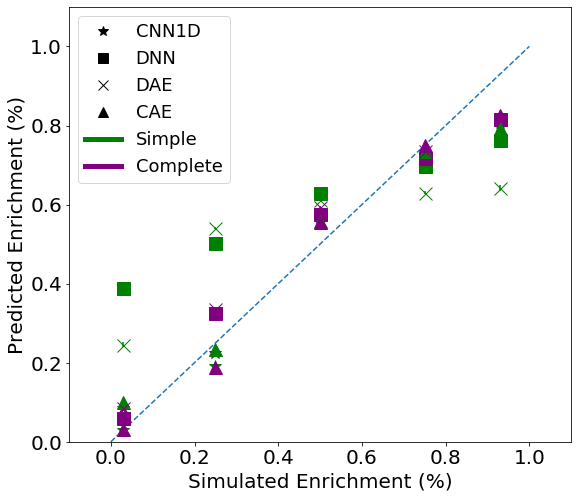
\includegraphics[width=\textwidth]{images/simuranium-noshield.png}
         \caption{Unshielded.}
         \label{fig:simuranium-noshield}
     \end{subfigure}
     \hfill
     \begin{subfigure}[b]{0.49\textwidth}
         \centering
         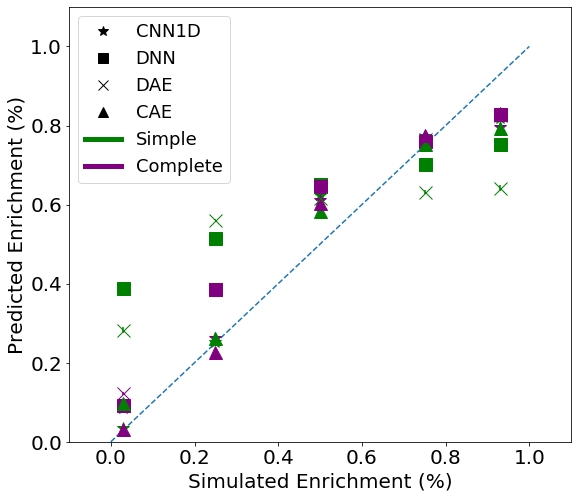
\includegraphics[width=\textwidth]{images/simuranium-lightal.png}
         \caption{1.48 cm aluminum.}
         \label{fig:simuranium-lightal}
     \end{subfigure}

     \begin{subfigure}[b]{0.49\textwidth}
         \centering
         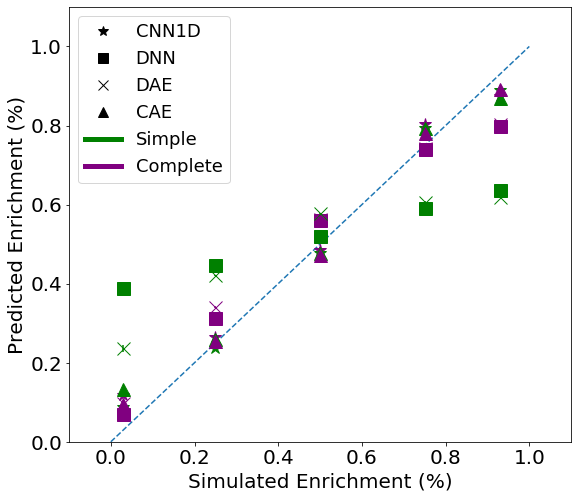
\includegraphics[width=\textwidth]{images/simuranium-mediumlead.png}
         \caption{0.450 mm lead.}
         \label{fig:simuranium-mediumlead}
     \end{subfigure}
     \hfill
     \begin{subfigure}[b]{0.49\textwidth}
         \centering
         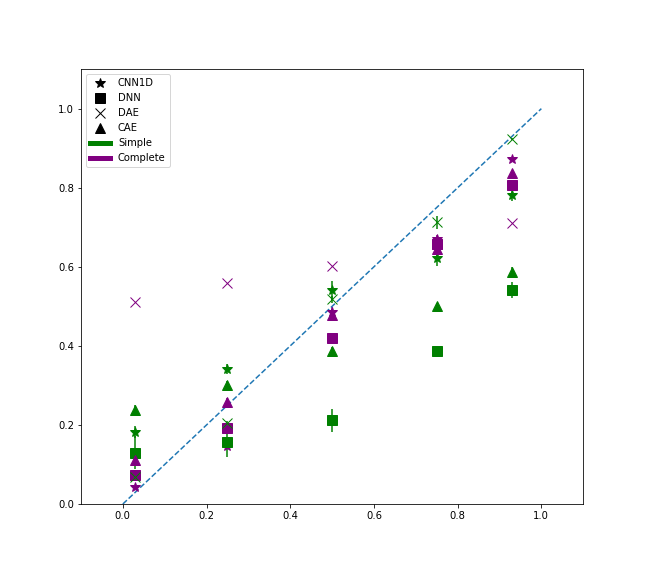
\includegraphics[width=\textwidth]{images/simuranium-heavylead.png}
         \caption{1.42 mm lead.}
         \label{fig:simuranium-heavylead}
     \end{subfigure}
        \caption{Shielding generalization performance in simulated enriched uranium spectra for the DNN, CNN with and without autoencoder pretraining. Simulated shielding amounts are indicated below each figure.} %Clockwise from the upper left, the shielding simulated are unshielded, 1.48 cm aluminum, 0.450 mm lead, and 1.42 mm lead.}
        \label{fig:simuranium-shielding}
\end{figure}


\begin{figure}[H]
	\centering
	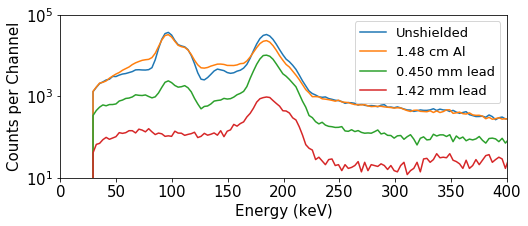
\includegraphics[width=0.8\linewidth]{images/simulated_uranium_shielding.png}
	\caption{Simulated 93\% enriched uranium spectra various amounts of shielding.}
	\label{fig:simulated_uranium_shielding}
\end{figure}


\subsection{Generalization Results on Changing Calibration}

To test each model's generalization performance with respect to calibration, enriched uranium spectra were simulated with various relative gains. The outputs from each model on these cases are shown in Figure \ref{fig:simuranium-cal}. Model performance at relative gains of 0.9 and 1.1 are similar to the case without a change in gains, shown in Figure \ref{fig:simuranium-noshield}.

At the extreme relative gain shifts of 0.8 and 1.2 performance for the models changes. At a relative gain shift of 0.8, the dense models display a large variance in output values while the convolutional models do not. Convolutional models are effected less by the large change in gain because of their inherent shift invariance. At a relative gain shift of 0.8, the 186 keV peak from $^{235}$U is shifted to the 225 keV region as seen in Figure \ref{fig:simulated_uranium_calibration_93pct}. In this region there is little spectral information about enrichment. Because of this, this peak - which is the main source of enrichment information - may be ignored. Because the 186 keV peak is ignored the dense networks underpredict enrichment at a 0.8 relative gain shift. At a gain shift of 1.2 each model overpredicts enrichment for enrichments at and below 50\%. Because the 1.2 relative shift moves the 766 keV and 1001 keV $^{238}$U peaks into regions of little importance for the spectra without gain shift, seen in Figure \ref{fig:simulated_uranium_calibration_10pct}, these peaks are ignored and the enrichment is overpredicted.

% Also, because the shifted peak is wider, more nodes connected to this region would need to update to extract useful information. 


\begin{figure}[H]
     \centering
     \begin{subfigure}[b]{0.49\textwidth}
         \centering
         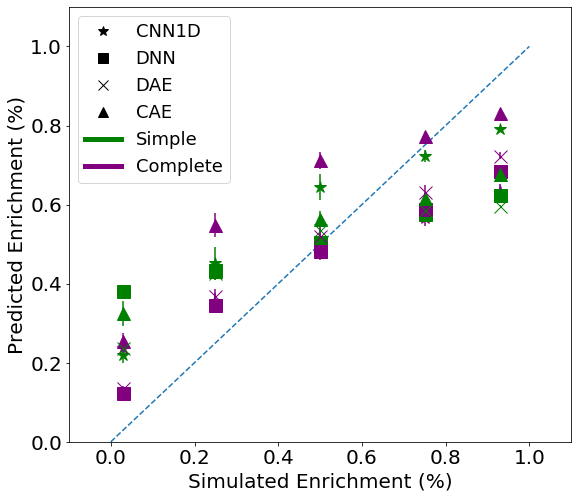
\includegraphics[width=\textwidth]{images/simuranium-cal08.png}
         \caption{0.8}
         \label{fig:simuranium-cal08}
     \end{subfigure}
     \hfill
     \begin{subfigure}[b]{0.49\textwidth}
         \centering
         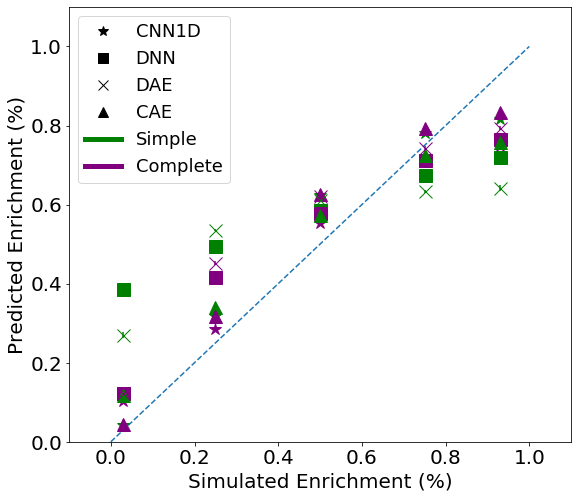
\includegraphics[width=\textwidth]{images/simuranium-cal09.png}
         \caption{0.9}
         \label{fig:simuranium-cal09}
     \end{subfigure}

     \begin{subfigure}[b]{0.49\textwidth}
         \centering
         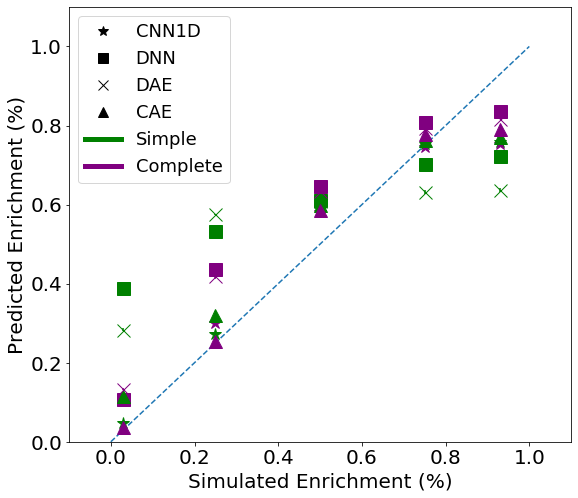
\includegraphics[width=\textwidth]{images/simuranium-cal11.png}
         \caption{1.1}
         \label{fig:simuranium-cal11}
     \end{subfigure}
     \hfill
     \begin{subfigure}[b]{0.49\textwidth}
         \centering
         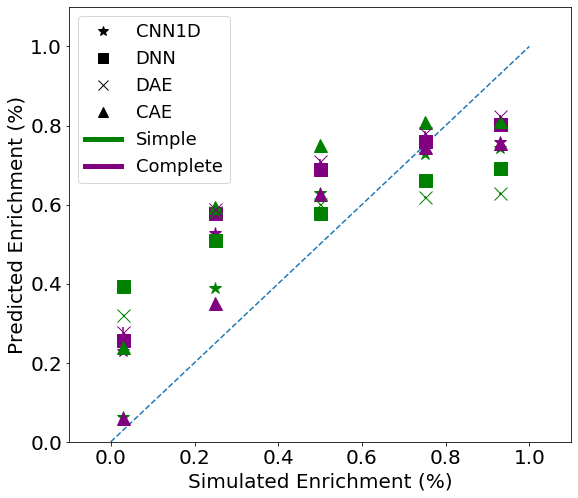
\includegraphics[width=\textwidth]{images/simuranium-cal12.png}
         \caption{1.2}
         \label{fig:simuranium-cal12}
     \end{subfigure}
        \caption{Calibration gain generalization performance in simulated spectra for the DNN, CNN with and without autoencoder pretraining. The magnitude of the applied relative gain shift are shown below each figure.}
        \label{fig:simuranium-cal}
\end{figure}





\begin{figure}[H]
	\centering
	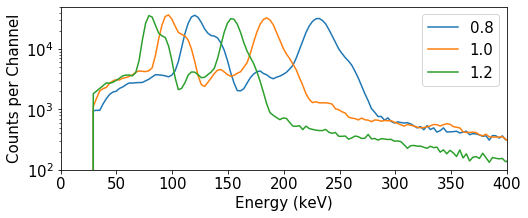
\includegraphics[width=0.8\linewidth]{images/simulated_uranium_calibration.png}
	\caption{Simulated 93\% enriched uranium spectra with three different relative gain settings. Energy calibration shown is based on the 1.0 relative gain setting.}
	\label{fig:simulated_uranium_calibration_93pct}
\end{figure}

\begin{figure}[H]
	\centering
	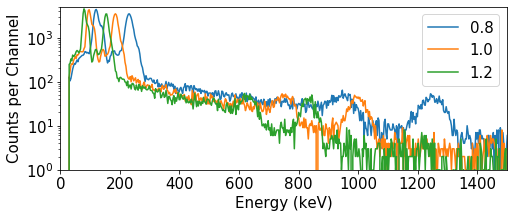
\includegraphics[width=0.8\linewidth]{images/simulated_uranium_calibration_1500kev.png}
	\caption{Simulated 10\% enriched uranium spectra with three different relative gain settings. Energy calibration shown is based on the 1.0 relative gain setting.}
	\label{fig:simulated_uranium_calibration_10pct}
\end{figure}

\section{Results - Measured Spectra}






\begin{figure}[H]
	\centering
	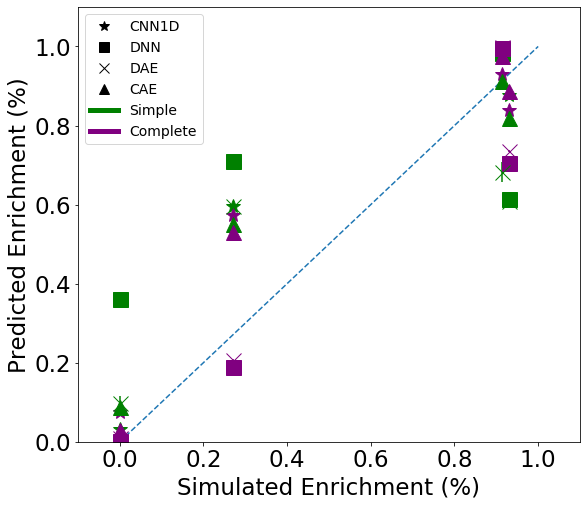
\includegraphics[width=0.8\linewidth]{images/measured_uranium.png}
	\caption{Results from measured uranium of different enrichments.}
	\label{fig:measured_uranium}
\end{figure}



\section{Discussion and Conclusion}

Other cases need to be added to the training dataset to make this work in practice. Additional examples need to $^{241}$Am, $^{239}$Pu, and $^{237}$Np from recycled uranium. 





